% !TEX TS-program = pdflatex
% !TEX encoding = UTF-8 Unicode

% This is a simple template for a LaTeX document using the "article" class.
% See "book", "report", "letter" for other types of document.

\documentclass[11pt]{article} % use larger type; default would be 10pt

\usepackage[utf8]{inputenc} % set input encoding (not needed with XeLaTeX)

%%% Examples of Article customizations
% These packages are optional, depending whether you want the features they
%provide.
% See the LaTeX Companion or other references for full information.

%%% PAGE DIMENSIONS
\usepackage{geometry} % to change the page dimensions
\geometry{a4paper} % or letterpaper (US) or a5paper or....
% \geometry{margins=2in} % for example, change the margins to 2 inches all round
% \geometry{landscape} % set up the page for landscape
%   read geometry.pdf for detailed page layout information

\usepackage{graphicx} % support the \includegraphics command and options

% \usepackage[parfill]{parskip} % Activate to begin paragraphs with an empty
%line rather than an indent

%%% PACKAGES
\usepackage{booktabs} % for much better looking tables
\usepackage{array} % for better arrays (eg matrices) in maths
\usepackage{paralist} % very flexible & customisable lists (eg.
%enumerate/itemize, etc.)
\usepackage{verbatim} % adds environment for commenting out blocks of text & for
%better verbatim
\usepackage{subfig} % make it possible to include more than one captioned
%figure/table in a single float
% These packages are all incorporated in the memoir class to one degree or
%another...

%%% HEADERS & FOOTERS
\usepackage{fancyhdr} % This should be set AFTER setting up the page geometry
\pagestyle{fancy} % options: empty , plain , fancy
\renewcommand{\headrulewidth}{0pt} % customise the layout...
\lhead{}\chead{}\rhead{}
\lfoot{}\cfoot{\thepage}\rfoot{}

%%% SECTION TITLE APPEARANCE
\usepackage{sectsty}
\allsectionsfont{\sffamily\mdseries\upshape} % (See the fntguide.pdf for font
%help)
% (This matches ConTeXt defaults)

%%% ToC (table of contents) APPEARANCE
\usepackage[nottoc,notlof,notlot]{tocbibind} % Put the bibliography in the ToC
\usepackage[titles,subfigure]{tocloft} % Alter the style of the Table of
%Contents
\renewcommand{\cftsecfont}{\rmfamily\mdseries\upshape}
\renewcommand{\cftsecpagefont}{\rmfamily\mdseries\upshape} % No bold!

%%% END Article customizations

%%% The "real" document content comes below...

\title{TeleScope-CF XML Content Filtering Engine Library Language  Specification}
\author{Kirill Belyaev, Palo Alto, CA, USA, 94306}
%\date{} % Activate to display a given date or no date (if empty),
         % otherwise the current date is printed 

\begin{document}
\maketitle

\section{Library Description and Query Composition}

	Current TeleScope-CF Java library implementation employs XML parsing and specific pattern-matching that provides standard logical operator constructs to construct the query over the values of XML elements and attributes applied to the XML message on the fly as it is provided in the form of a String object.
	
	The code base has been adopted from TeleScope CQ XML stream broker code base written in C. C code has been re-factored into Java with minor modifications. 

This general-purpose library could be used by any Java applications that are involved in the XML message content filtering. Example application scenarios could be intrusion detection, selective rule engines, targeted database insertions during the ETL process and various business logic scenarios.  The library could also be used in XML routers and various web services for XML content filtering where XML is a common message passing format.   

The engine library could accept either a single query or a set of queries.

The query could be constructed out of a number (two and more) of simple sub-queries (expressions) connected via either a logical \textbar \space OR operator or a logical \& \space AND operator. 

A query can not have both logical operators in it at the same time.
Therefore queries could be composed either of:

\begin{itemize}
\item{sub-queries chained via \textbar \space OR logical operators}
\item{sub-queries chained via \& \space AND logical operators}
\end{itemize}


This model provides the ability to perform query decomposition and construct a complex query in the form of individual sub-queries submitted to the engine as a query set. This approach allows to eliminate the need for parentheses () between sub-queries for the sake of query simplification. 

For example the query 

\begin{itemize}

\item{ "(type = STATUS \textbar \space ORIGIN = EGP) \textbar \space (type = UPDATE \& MULTI\_EXIT\_DISC = 100 \& SRC\_AS = 6447 \& SRC\_PORT = 4321 \& ORIGIN = EGP) \textbar \space (MULTI\_EXIT\_DISC = 10 \& SRC\_AS = 6447 \& SRC\_PORT = 4321 \& ORIGIN = EGP) \textbar \space (type = KEEPALIVE \& DST\_AS \textgreater 3200)" }

\end{itemize}

will be decomposed into several sub-queries each of which will be presented as a separate query to the engine in the form of a query set:

\begin{itemize}

\item{type = STATUS \textbar \space ORIGIN = EGP}

\item{type = UPDATE \& MULTI\_EXIT\_DISC = 100 \& SRC\_AS = 6447 \& SRC\_PORT = 4321 \& ORIGIN = EGP}

\item{MULTI\_EXIT\_DISC = 10 \& SRC\_AS = 6447 \& SRC\_PORT = 4321 \& ORIGIN = EGP}

\item{type = KEEPALIVE \& DST\_AS \textgreater 3200}

\end{itemize}

Here we provide the sample use cases of valid and invalid query expressions inputs:

\begin{itemize}

\item{"type = STATUS \textbar \space type = UPDATE" - valid query expression
chained via  a logical \textbar \space OR operator}

\item{"type = STATUS \textbar \space type = UPDATE \textbar \space type =
KEEPALIVE" - valid query expression chained via  a logical \textbar \space OR
operator}


\item{"type = STATUS \& \space type = UPDATE \& SRC\_AS = 6447" - valid query
expression chained via  a logical \& \space AND operator}

\item{"type = UPDATE \& MULTI\_EXIT\_DISC = 100 \& SRC\_AS = 6447 \& SRC\_PORT =
4321 \& ORIGIN = EGP" - valid query expression chained via a logical \& \space
AND operator }


\item{"type = STATUS \textbar \space type = UPDATE \& SRC\_AS = 6447" - invalid query expression - usage of both logical AND/OR operators is ambiguous and therefore prohibited in a single query. This query could be submitted to the engine in the form of two separate sub-queries - one with OR operator logic and second with AND operator logic}

\end{itemize}

The TeleScope-CF Library Language operators are presented in the  Table
\ref{table:language operators} with sample use cases\label{table:language
operators}:

\begin{table}[ht] 
\caption{TeleScope-CF Library Language operators } % title of Table 
\label{table:language operators}
\centering      % used for centering table 
\begin{tabular}{c c c}  % centered columns (3 columns) 
\hline\hline                        %inserts double horizontal lines 
Operator & Description & Example use \\ [0.25ex] % inserts table 
%heading 
\hline                    % inserts single horizontal line 
=  & equality operator & ORIGIN = EGP \\   % inserting body of the table 

! & not-equal operator & SRC\_AS ! 6447 \\

\textless  & relational less than operator & MULTI\_EXIT\_DISC \textless 10 \\

\textgreater  & relational greater than operator & MULTI\_EXIT\_DISC
\textgreater 10 \\

\& & logical AND  &  ORIGIN = EGP \& value = 0 \\

\textbar \space & logical OR & ORIGIN = EGP \textbar \space value = 1 \\

\%  & substring match & type \% AS\_S \\ [1ex] %[1ex] adds vertical space 
\hline     %inserts single line 
\end{tabular} 
\label{table:language operators}  % is used to refer  to this table in the text 
\end{table} 

Equality and negation operators (= and !) could be used in expressions involving both string and integer values and change the semantics of operation depending on operand type. Full text search functionality is not yet incorporated in the current release of the library. A subset of this functionality is included through \% substring match operator.

TeleScope-CF provides a set of operators designed specifically for processing
network prefixes including CIDR ranges.  The operators follow the designated network prefix element (in our example it is the PREFIX attribute within the BGP XML Message) with the subsequent network range value. These are ordinary English letters having special meaning when used within the expression\label{table:network prefix operators}.


\begin{table}[ht] 
\caption{Network prefix (CIDR) operators } % title of Table 
\centering      % used for centering table 
\begin{tabular} %{c c c}  % centered columns (3 columns) 
{ | l | l | l | p{5cm} |}
\hline\hline                        %inserts double horizontal lines 
Operator & Description & Example use & Semantics \\ [0.25ex] % inserts table 
%heading 
\hline                    % inserts single horizontal line 
e  & exact prefix match operator & PREFIX e 211.64.0.0/8 & exactly defined 

network prefix range. \\ \hline

l  & less specific prefix match operator & PREFIX l 211.64.0.0/8 & less specific


network prefix range. \\ \hline

m & more specific prefix match operator & PREFIX m 211.64.0.0/8 & more specific 

network prefix range.  \\ \hline
\end{tabular} 
\label{table:network prefix operators}  % is used to refer  to this table in the text 
\end{table} 

The network prefix processing operators are not included in the current release of the library.


\begin{figure}[!htb]
\centering
\scalebox{0.6}{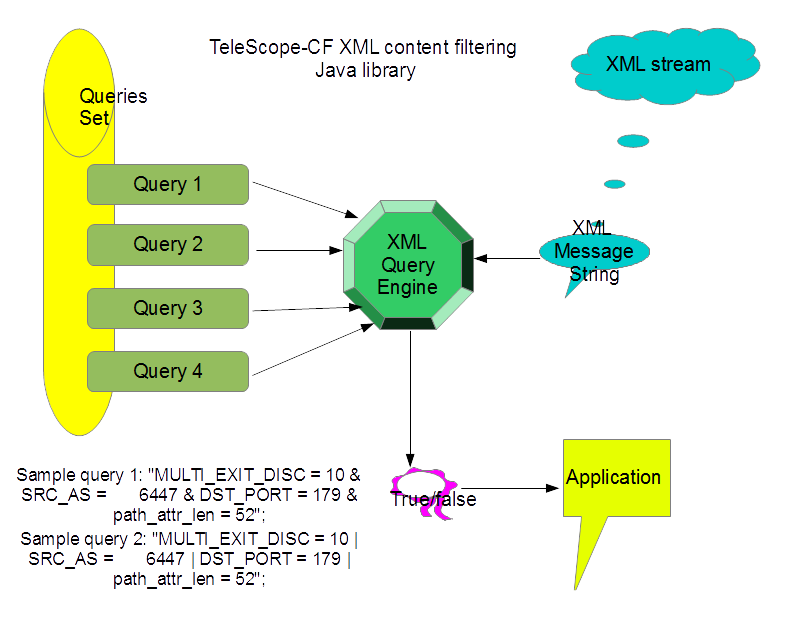
\includegraphics{telescope-cq-lib.png}}
\caption{ TeleScope-CF Library Architecture}
\label{TeleScope-CF Library}
\end{figure}



\section{Example Java library usage interface}

Java library is provided as a jar file that should be imported by the targeted application for XML content filtering:

import static iface.Constants.DefaultArraySize;

import implementation.*;

String Query = "MULTI\_EXIT\_DISC = 10 \& SRC\_AS = 6447 \& DST\_PORT = 179 \&
path\_attr\_len = 52";

Engine engine = new Engine();

engine.addQuery(Query);

boolean result = engine.runQueries(XMLmessage);
		
System.out.println("query returned " + result);

engine.deleteQueries();


More then one Query could be added via the addQuery() method for a specified XML message string. Any query that evaluates to true would make engine terminate and return true. If none of the registered queries evaluates to true the engine will return false to the calling application.   

\end{document}